\documentclass[11pt]{article}
\usepackage[a4paper,margin=1in]{geometry}
\usepackage[T1]{fontenc}
\usepackage[utf8]{inputenc}
\usepackage{lmodern}
\usepackage{microtype}
\usepackage{booktabs}
\usepackage{tabularx}
\usepackage{graphicx}
\usepackage{enumitem}
\usepackage{caption}
\usepackage{xcolor}
\usepackage[colorlinks=true,linkcolor=black,urlcolor=blue!55!black,citecolor=black]{hyperref}
\setlist{itemsep=2pt,topsep=4pt,parsep=0pt}
\captionsetup{font=small,labelfont=bf}
\setlength{\parskip}{5pt}
\setlength{\parindent}{0pt}
\newcommand{\N}{N}

\title{\textbf{Do Their Numbers Match? An Auditable Dataset of Statistical Claims in Nigerian National Addresses}}
\author{Mia\\ \small Independent}
\date{\small AI $\times$ Epistemics Research Sprint, 13--15 November 2026\\ Track 4: Open Track (deployment, adoption and impact)}

\begin{document}
\maketitle
\vspace{-1.2em}

\begin{abstract}
\noindent
Tools that check public claims against official statistics need ground truth: claims paired with the release they cite and a verdict. Almost none exists for Nigeria. This project builds a first open dataset. Every figure in five scripted national addresses delivered between October 2025 and October 2026 was listed: four by President Bola Tinubu and one by opposition candidate Atiku Abubakar. That gave 51 figures. Thirty-one were checked against releases from the statistics bureau, the central bank, the debt office and other official bodies, and 29 could be scored. Of those, 20 matched the official figure (69\%), 5 were close (17\%) and 4 did not match (14\%). The nine errors were not uniformly self-serving: five favoured the speaker's argument and four cut against it. They fall into recognisable types. A definition was swapped (``non-oil'' exports of 48\% that are mostly petroleum products and gas; exports outside oil and gas were about 13\%). Figures were stale (a stock-market gain quoted from ten days earlier). A baseline month was misattributed. One claim matched one official source while a second official source gave less than half the amount. One could not be checked because only the government's own statement exists. The dataset, with a source link on every scored row, is public. It is small, was checked by an AI assistant without a second checker, and relies mostly on press reports of official releases; these limits are stated in full.
\end{abstract}

\section{Introduction}

A large share of political argument is carried by numbers: growth, inflation, reserves, prices. In principle these are the easiest claims to check, because an official release exists for each. In practice the checking is slow, and for many countries nobody has assembled the claims and the releases side by side in a form that can be audited or reused.

This matters for AI. Systems that verify claims, and the benchmarks that test them, are built mostly on material from a few countries with accessible statistics and established fact-checking outlets. A model evaluated only there tells us little about how it will do where official figures are published as PDFs, where two agencies report different numbers for the same quantity, and where a claim may rest on a government statement with no release behind it. The sprint brief asks for exactly this: pair quantitative claims with the statistical releases they cite, flag mismatches with links, and publish an auditable dataset.

This project does that for Nigeria, at small scale. Its contributions are: (i) an open dataset of 51 figures from five national addresses, 29 of them scored against official releases with a link on each; (ii) a typology of how the figures went wrong, drawn from the data; (iii) evidence that the errors were not uniformly self-serving; and (iv) two cases that a simple match/mismatch scheme cannot represent, which any automated checker will need to handle.

\section{Related Work}

Fact-checking organisations in Nigeria, including Africa Check and Dubawa, publish verdicts on individual claims, chosen for newsworthiness. This project differs in sampling: it lists every figure in a defined set of speeches and reports how many were checked, so the denominator is visible. In the United Kingdom, Full Fact and the Office for Statistics Regulation perform a similar function with far better-resourced statistical infrastructure.

The sprint's framing documents argue that governments lag in adopting epistemic tools \cite{vaintrob_gap} and name the failure of good tools to be adopted as an open problem \cite{vaintrob_tools}. Public datasets such as Community Notes \cite{chuai} show what an auditable record of contested claims can support. This dataset is a much smaller contribution of the same kind, for a setting those resources do not cover.

\section{Methodology}

\subsection{Sample}

Five scripted national addresses whose full texts are published were selected before any checking: President Tinubu's Independence Day broadcast (1 October 2025), 2026 budget speech (19 December 2025), New Year message (1 January 2026) and Independence Day address (1 October 2026); and Atiku Abubakar's Independence Day address, delivered the same morning as the last of these. Including the main opposition candidate means government and opposition are checked by the same procedure.

\subsection{Extraction}

Every sentence containing a figure about the economy or public finances was listed from each text. Figures that are proposals or targets were excluded, as were historical figures with no current official series. This gave 51 figures: 41 from the President's four addresses and 10 from the opposition address.

\subsection{Checking}

For each figure the checker looked for the official release it refers to: the National Bureau of Statistics (GDP, prices, trade, capital importation), the Central Bank of Nigeria (reserves, balance of payments), the Debt Management Office, the upstream petroleum regulator, the student loan fund, the export promotion council and the tax authority. Each figure received one verdict:

\begin{itemize}
\item \textbf{Match:} the official figure agrees with the claim.
\item \textbf{Close:} the claim is within rounding, or within roughly ten to fifteen per cent, of the official figure.
\item \textbf{Mismatch:} the official figure differs materially, or the claim describes a different quantity from the one named.
\item \textbf{Unverifiable:} no release could be found beyond the speaker's own side repeating the figure.
\item \textbf{Forecast:} a prediction when spoken; recorded with its outcome but not scored.
\item \textbf{Not checked:} listed, but not reached in the time available.
\end{itemize}

Each error was also given a type, and a direction: \emph{favourable} if the error strengthens the speaker's argument and \emph{unfavourable} if it weakens it.

Thirty-one figures were checked. Checking was prioritised by prominence (headline growth, inflation, reserves, trade and debt first), not sampled at random, so the match rate describes the checked figures and should not be read as the rate for all 51.

\subsection{Who did the checking}

All extraction and checking was done by an AI assistant (Claude, Anthropic) using web search, directed by the author. There was no second checker. Three figures were verified against the primary document. Of the other 26 scored figures, 25 were verified through press reports that quote the official release and one against the tax authority's own statement, with the source linked on the row. Section~\ref{sec:limits} sets out what this means for reliability.

\section{Results}

\subsection{Most checked figures matched}

\begin{figure}[h]
\centering
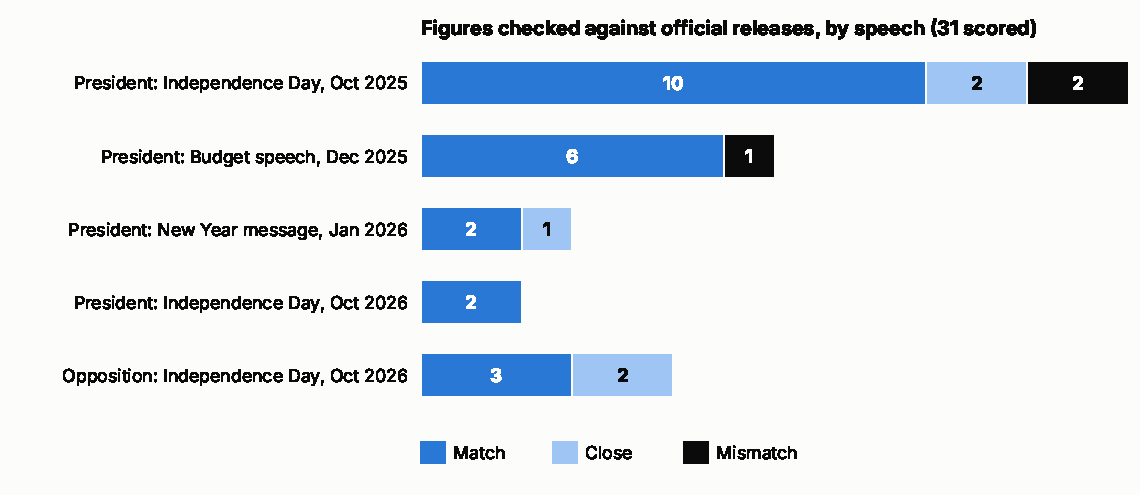
\includegraphics[width=0.9\linewidth]{figure1.pdf}
\caption{Verdicts on the 29 scored figures, by speech.}
\label{fig:verdicts}
\end{figure}

Of the 31 figures checked, 29 could be scored: 20 matched (69\%), 5 were close (17\%) and 4 did not match (14\%). One was unverifiable and one was a forecast (Table~\ref{tab:verdicts}). Headline macroeconomic figures were reliable: every quarterly GDP growth rate and monthly inflation rate quoted in the five speeches matched the statistics bureau's release exactly.

\begin{table}[h]
\centering
\small
\setlength{\tabcolsep}{4pt}
\begin{tabular}{lccccccc}
\toprule
 & Listed & Match & Close & Mismatch & Unverif. & Forecast & Unchecked \\
\midrule
President Tinubu (4 addresses) & 41 & 17 & 3 & 4 & 1 & 1 & 15 \\
Atiku Abubakar (1 address) & 10 & 3 & 2 & 0 & 0 & 0 & 5 \\
\midrule
Total & 51 & 20 & 5 & 4 & 1 & 1 & 20 \\
\bottomrule
\end{tabular}
\caption{All 51 listed figures by verdict.}
\label{tab:verdicts}
\end{table}

The two speakers cannot be compared from these counts. They gave different numbers of speeches, of different kinds, and different shares of their figures were checked.

\subsection{How the figures went wrong}

The four mismatches and five close calls fall into four types.

\textbf{A definition was swapped.} The October 2025 broadcast said non-oil exports ``now represent 48 per cent, compared to oil exports, which account for 52 per cent''. The trade release for that quarter shows crude oil at 52.6\% of exports, but a further 34.2\% was other petroleum products and gas. Exports outside oil and gas were about 13\%. The 48\% is ``everything except crude'', presented as ``non-oil''. This is the most consequential error in the set, because the claim is about diversification away from oil.

\textbf{A baseline was misattributed or understated.} The same broadcast said oil output had recovered ``from barely one million [barrels a day] in May 2023''. The regulator recorded 1,183,691 barrels a day of crude in May 2023; the figure near one million (998,602) was April. The tax-to-GDP ratio was said to have risen ``from less than 10 per cent''; the tax authority had reported 10.86\% for 2022. The opposition address put a sliced loaf at ``about \N 500'' in April 2023; the statistics bureau's average was \N 561.21. In each case the lower starting point makes the change look larger.

\textbf{Figures were stale.} The New Year message said the stock market had gained 48.12\% in 2025. That was the year-to-date return on 22 December; the full-year return was 51.19\%. The budget speech said ``over 418,000'' students had been supported by the loan fund, although the fund had reported 510,378 beneficiaries in September and the President had cited about 510,000 eleven weeks earlier. Both errors understate the speaker's own case.

\textbf{Rounding.} Reserves of \$46.7 billion were given as ``about US\$47 billion''; an upkeep allowance of \N 45.7 billion as \N 44.7 billion.

\subsection{The errors were not uniformly self-serving}

Of the nine errors, five favoured the speaker's argument and four cut against it (President: 4 and 3; opposition: 1 and 1). The opposition address said a \N 70,000 minimum wage ``buys just 50 litres'' of petrol; at the latest official price found (\N 1,596.25 in May 2026) it buys about 44, so the claim understated the speaker's own point. A pattern of deliberate inflation would not produce this mix. Stale briefing notes and loose definitions would.

\subsection{Two cases a match/mismatch scheme cannot hold}

\textbf{Two official sources disagree.} The New Year message said foreign direct investment ``rose to \$720 million, up from \$90 million in the preceding quarter''. The central bank's balance of payments for the third quarter of 2025 gives exactly these figures. The statistics bureau's capital importation report for the same quarter gives \$296.25 million, up from \$142.67 million. The two series measure different things (the bureau's counts fresh capital entering through banks and excludes reinvested earnings), but both are official and both are called FDI. The claim is scored as a match, and the row records the conflict. A checker with access to only one series would return a confident verdict either way.

\textbf{No release exists.} The October 2025 broadcast said the debt service-to-revenue ratio had fallen ``from 97\% to below 50\%''. The only sources found were statements by the President and the head of the tax authority. A year earlier the President had given the ratio as 65\%. Without a published series the claim cannot be confirmed or refuted from public records.

\section{Discussion}

\textbf{What this suggests for claim-checking tools.} The easy cases here are very easy: a named statistic for a named period, published once. A system that only handled those would have scored most of this set correctly. The cases that matter are the others. Catching the non-oil export claim requires knowing that the released category is ``crude oil'', not ``oil'', and reading the breakdown. Catching the oil baseline requires checking the month. The FDI case requires knowing that two official series exist. None of these is solved by retrieving a number and comparing it.

\textbf{What this suggests for those who write the speeches.} Two of the four mismatches would have been avoided by using the latest figure. Both understated the government's own record.

\textbf{What the dataset is for.} Each row gives the claim, the speech, the official figure, the source, a verdict, an error type and a direction. That is enough to use the scored rows as a small test set for claim-verification systems in a low-resource statistical setting, and the 20 unchecked rows are open tasks. It is a starting point, and it should be extended and independently re-checked before anyone relies on it.

\section{Conclusion}

Across five Nigerian national addresses, 29 figures were scored against official releases. About seven in ten matched, and headline growth and inflation figures were quoted accurately every time. The errors that did occur were mostly stale figures, loose baselines and one swapped definition, and they did not consistently favour the speaker. Two claims exposed limits in the idea of a single official number. The dataset is public, with a link on every scored row, so that each verdict can be checked.

\begin{thebibliography}{9}\small
\bibitem{vaintrob_gap} L. Vaintrob. The AI Adoption Gap. Forethought, 2025. \url{https://www.forethought.org/research/the-ai-adoption-gap}
\bibitem{vaintrob_tools} L. Vaintrob and O. Cotton-Barratt. AI Tools for Existential Security. Forethought, 2025. \url{https://www.forethought.org/research/ai-tools-for-existential-security}
\bibitem{chuai} Y. Chuai et al. Did the Roll-Out of Community Notes Reduce Engagement With Misinformation? CSCW, 2024. \url{https://arxiv.org/abs/2307.07960}
\bibitem{tally} Tally: the dataset, analysis script and this report. \url{https://github.com/Mhiah/Tally}
\end{thebibliography}

\appendix

\section{Limitations and Dual-Use / Ethical Considerations}
\label{sec:limits}

\subsection*{Limitations}

\begin{itemize}
\item \textbf{Small and incomplete.} Five speeches, 51 figures, 29 scored. Twenty listed figures were not checked.
\item \textbf{Checked figures were not chosen at random.} Prominent figures were checked first. The 69\% match rate applies to the checked set only.
\item \textbf{A single AI checker.} One AI assistant did the extraction and checking, with no second checker and no human verification of each row. Errors in the dataset are possible. Every scored row carries a link so that the verdict can be audited.
\item \textbf{Mostly secondary sources.} Only 3 of the 29 scored figures were verified against the primary document. The rest rely on press reports quoting the official release, and one on an agency's own statement. Where several outlets reported the same figure this is low-risk, but it is not the same as reading the release.
\item \textbf{Extraction relied on published transcripts,} which may differ from the speech as delivered, and was done with a tool that truncates long quotations, so claim wording in the dataset is sometimes an excerpt.
\item \textbf{Verdict thresholds are judgement calls.} ``Close'' and ``mismatch'' are separated by a rough ten to fifteen per cent rule, and the direction labels reflect the checker's reading of each speaker's argument.
\item \textbf{The speakers are not comparable.} Four speeches against one, of different kinds, with different shares checked.
\item \textbf{Official figures are taken as the reference,} not as truth. Official statistics can themselves be wrong or revised; several series here were rebased during the period.
\end{itemize}

\subsection*{Dual-use and ethical considerations}

\begin{itemize}
\item \textbf{Political use.} The dataset covers a sitting president and an opposition candidate ahead of an election year. It could be quoted selectively by either side. The safeguards are symmetry (one procedure for both), a visible denominator (all 51 figures are listed, including the unchecked ones) and the finding itself, which is that most checked figures matched and errors ran in both directions.
\item \textbf{Named individuals.} The claims are public statements by public figures in their official capacity. No private information is used.
\item \textbf{False authority.} A dataset with verdicts can look more settled than it is. This one was built in a weekend by an AI assistant and has not been independently re-checked. It should not be cited as a fact-check of record.
\item \textbf{Over-reading.} The results do not show that either speaker is more or less honest than the other, and they say nothing about claims that contain no figures.
\end{itemize}

\subsection*{AI assistance and prior work}

An AI assistant (Claude, Anthropic) did the web research, the checking, the analysis script and the drafting of this report, under the author's direction. The author is responsible for the content. Nothing here existed before the sprint.

\subsection*{Reproducibility}

The dataset is \texttt{data/claims.csv} in the repository \cite{tally}. Every count in this report is produced by \texttt{analyze.py} from that file. The verification log kept during checking is \texttt{notes.md}.

\end{document}
